\chapter{Аппаратная платформа и алгоритм проведения измерений}
	
Управляющее устройство реализовано на базе ПЛИС, так как есть необходимость разрабатывать 
специфические аппаратные модули.\\

В качестве аппаратной платформы УУ (управляющее устройство) выступает ПЛИС серии
LittleBee китайского производителя Gowin Semiconductor -- GW1N-UV9QN88C6/I5.\\

\noindent Данная ПЛИС имеет следующие характеристики:\\


\begin{itemize}
	\item количество логических блоков LUT4 -- 8640 шт.
	\item количество триггеров -- 6480 шт.
	\item объём FLASH -- 408 Кбит
	\item количество блоков BSRAM -- 26 шт.
	\item объём блоков SRAM -- 468 Кбит
	\item количество блоков PLL (ФАПЧ) -- 2 шт.
	\item напряжение питания ядра -- 1.8–3.3 В
	\item количество доступных для пользователя выходов I/O -- 77
	\item среди них дифференциальных пар -- 19\\
\end{itemize}

\begin{figure}[ht!] 
	\center
	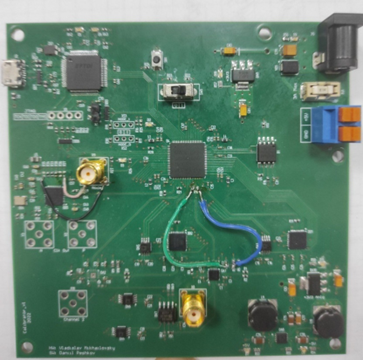
\includegraphics {my_folder/images//pcb}
	\caption{Печатная плата устройства} 
	\label{fig:pcb}  
\end{figure}

\begin{figure}[ht!] 
	\center
	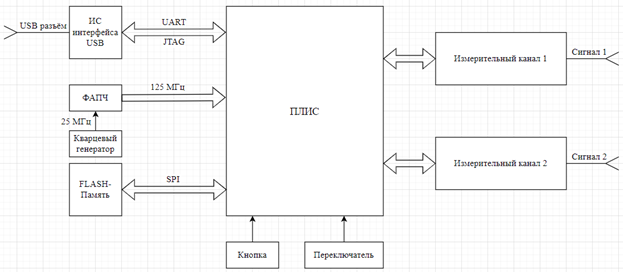
\includegraphics {my_folder/images//scheme_struct}
	\caption{Структурная схема устройства} 
	\label{fig:scheme-struct}  
\end{figure}

На \firef{fig:scheme-struct} изображена структурная схема устройства.
К УУ подключаются два измерительных канала, которыми необходимо управлять для проведения измерений.
ПЛИС тактируется высокостабильным тактовым сигналом с частотой 125 МГц. Связь с устройством верхнего уровня
осуществляется через FTDI чип FT2232H.

Перед разработкой УУ необходимо определить ОУ (объект управления), которым предстоит управлять.

\section{Измерительный канал}

\begin{figure}[ht!] 
	\center
	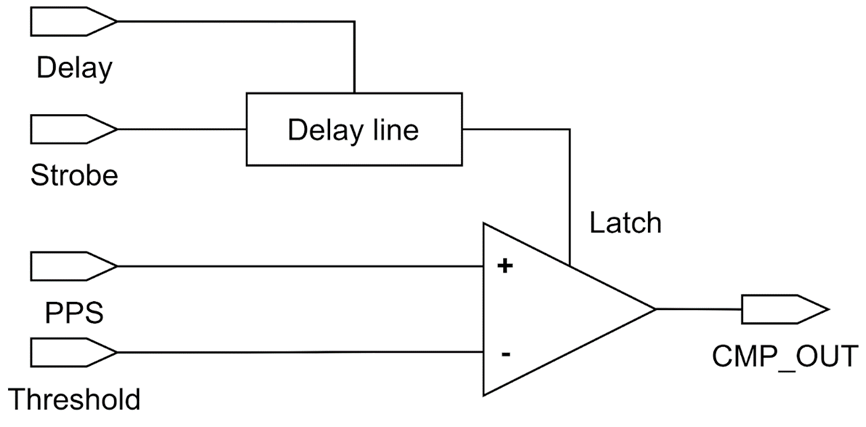
\includegraphics {my_folder/images//ch_func}
	\caption{Функциональная схема измерительного канала} 
	\label{fig:ch-func}  
\end{figure}

На \firef{fig:ch-func} приведена функциональная схема одного из измерительных каналов.


\begin{itemize}[label={}]
	\item Threshold -- пороговое напряжение сравнения на компараторе
	\item Delay -- настройка задержки сигнала на линии задержки (Delay line)
	\item Strobe -- стробы, выдаваемые УУ и защёлкивающее текущий результат сравнения компаратора.
	\item PPS -- измеряемый сигнал 1-PPS (В общем случае, может быть любой частоты, кратной либо 125 МГц,
		либо частоте внешнего тактового сигнала, подаваемого с SMA разъёма)\\
\end{itemize}

\section{Алгоритм проведения измерений}

Перед началом проведения измерения необходимо определить частоты измеряемого сигнала и найти его фронт.

\begin{figure}[ht!] 
	\center
	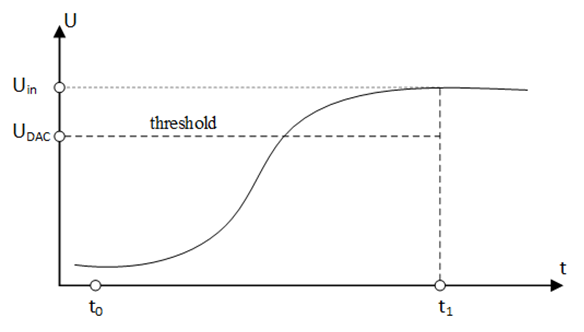
\includegraphics {my_folder/images//meas_alg}
	\caption{Измерение сигнала} 
	\label{fig:meas-alg}  
\end{figure}

Далее необходимо начать генерировать стробы с частотой измеряемого сигнала. Стробы блокируют
текущий выход компаратора, и на его выходе остаётся результат сравнения в момент прихода стробы.
При помощи изменения задержки можно сдвигать измеряемую точку по оси OX.
Для поиска значения напряжения в измеряемой точке необходимо изменять пороговое напряжение сравнения
на компараторе.

На \firef{fig:meas-alg} приведён пример измерения. 
$ t_{0} $ -- точка от которой измеряется сигнал (момент прихода стробы),
$ t_{1} $ -- измеряемая точка (момент прихода задержанной стробы на компаратор).
Временной отрезок $ [t_{0}, t_{1}] $ задаётся линией задержки.
Если в момент защёлкивания на выходе компаратора логическая единица, значит измеряемое напряжение выше,
чем пороговое. Перед приходом следующей стробы пороговое напряжение повышается.
Так продолжается до тех пор, пока на выходе компаратора не будет логического нуля.
В таком случае мы считаем, что измеряемая точка имеет значения напряжение равное пороговому.
Задержка увеличивается, и измеряется следующая точка. Таким образом снимается осциллограмма входного сигнала.


\section{Пороговое напряжение сравнения}
%НУ ТАКОЕ

Для задания порогового напряжения используется DAC (Digital to analog converter) AD5662 от Analog Devices.
AD5662 -- 16-битный DAC с гарантированной точностью 12 бит.

%\begin{figure}[ht!] 
%	\center
%	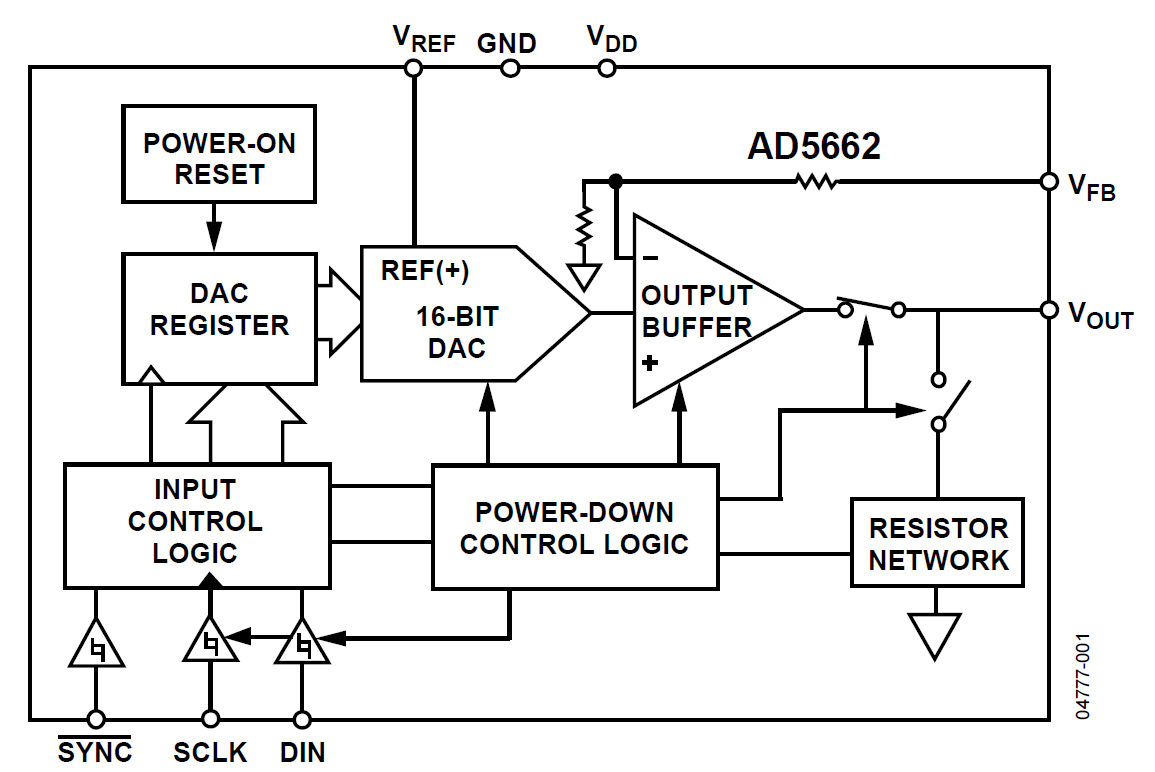
\includegraphics [scale=0.5] {my_folder/images//dac_func}
%	\caption{Функциональная схема AD5662} 
%	\label{fig:dac-func}  
%\end{figure}

С опорным напряжением 3.3 В, шаг изменения напряжения -- $ \frac{3.3}{2^{16}} \approx 50 $ мкВ.
Для задания напряжения используется интерфейс SPI (\firef{fig:dac-interface}).

\begin{figure}[ht!] 
	\center
	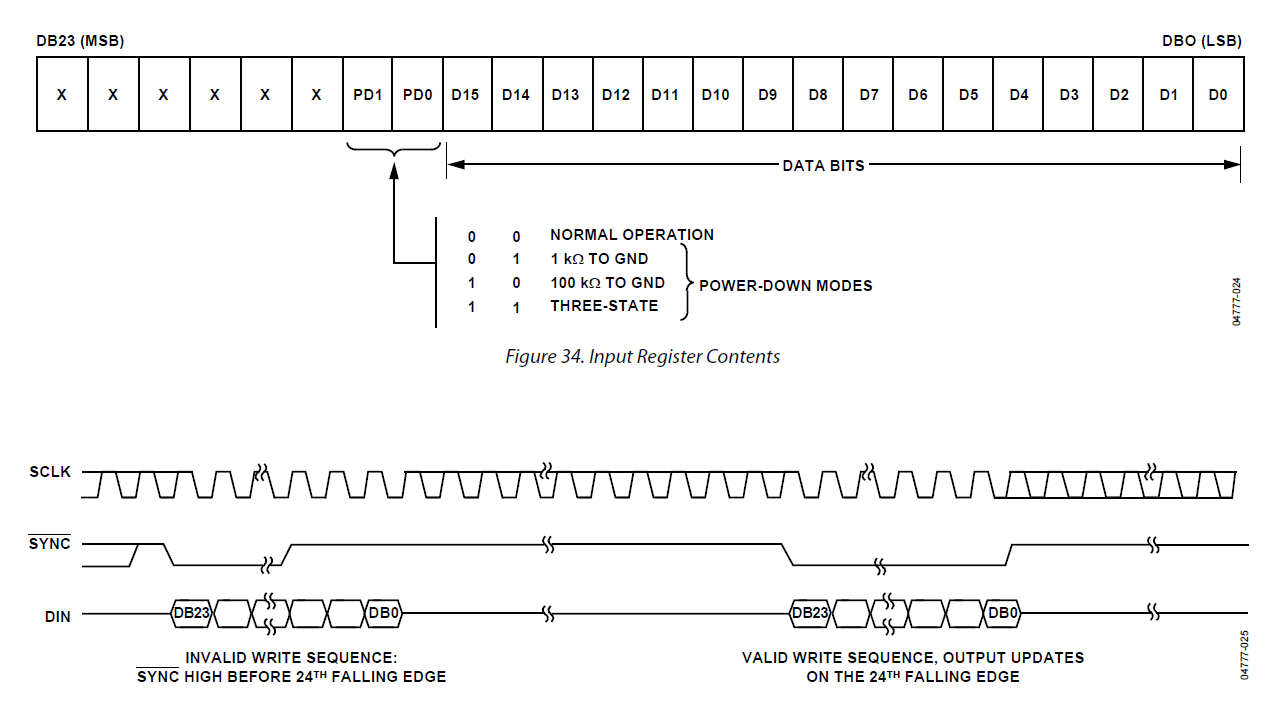
\includegraphics [scale=0.5] {my_folder/images//dac_interface}
	\caption{Интерфейс взаимодействия с AD5662} 
	\label{fig:dac-interface}  
\end{figure}

При напряжении питания 3.3 В максимальная частота сигнала SCLK -- 20 МГц. Максимальное время установки
выходного напряжения -- 10 мкс (обычно 8 мкс).

\section{Линия задержки}

Для сдвига задержки строба используется микросхема SY100EP196V от Microchip. Задержка задаётся 10-битным
цифровым кодом с шагом $ \approx $ 10 пс (\firef{fig:dline-code}). Так же есть аналоговый вход FTUNE, которым можно точнее точнее подстраивать
задержку (\firef{fig:dline-ftune}) (на данный момент не используется).

\begin{figure}[ht!] 
	\center
	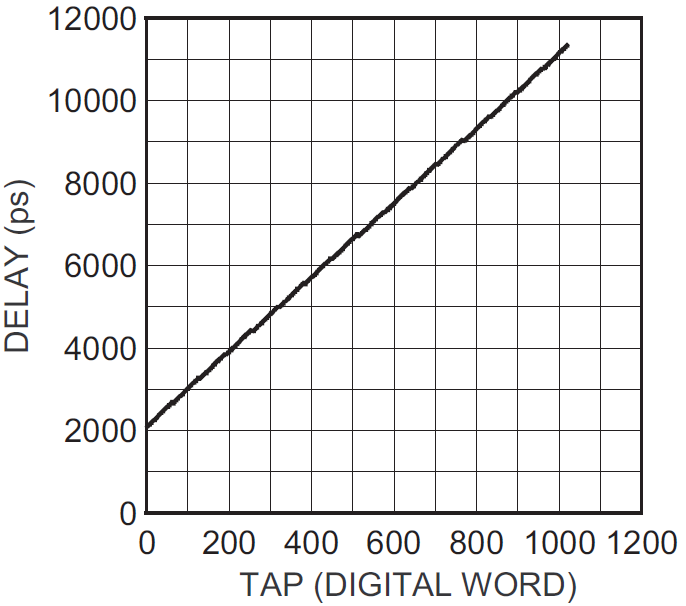
\includegraphics [scale=0.6] {my_folder/images//dline_code}
	\caption{Задержка, задаваемая цифровым входом} 
	\label{fig:dline-code}  
\end{figure}

\begin{figure}[ht!] 
	\center
	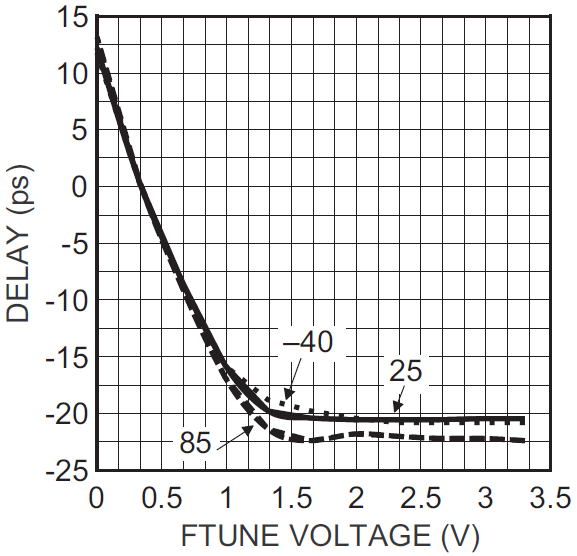
\includegraphics [scale=0.6] {my_folder/images//dline_ftune}
	\caption{Подстройка задержки через аналоговый вход FTUNE} 
	\label{fig:dline-ftune}  
\end{figure}


\section{Компаратор}

Для сравнения используется компаратор ADCMP582 от Analog Devices. Основным параметром, который необходимо учесть является $ t_{PL} $ (\firef{fig:cmp-wave}).

\begin{figure}[ht!] 
	\center
	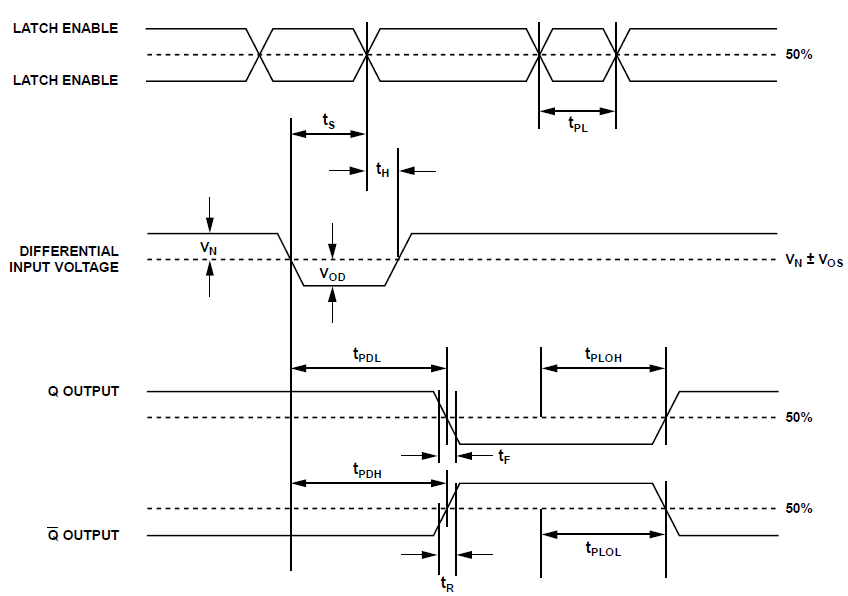
\includegraphics [scale=0.7] {my_folder/images//cmp_wave}
	\caption{Временная диаграмма ADCMP582} 
	\label{fig:cmp-wave}  
\end{figure}
\FloatBarrier

$ t_{PL} $ -- минимальное время, в течение которого сигнал защёлки (Latch Enable) должен быть высоким, чтобы получить результат сравнения попал на выход компаратора.

\newpage